\section{Transformation rules}\label{tr}





\subsection{LAM property definition}

	This section explains how to generate an OWL definition of a data and object property by transformation of a \textit{lam:DocumentProperty}. Figure \ref{fig:mapping-property-data} provides a visual representation of the mapping rules from a source lam:DocumentProperty on the left to a target owl:DataProperty (or owl:ObjectProperty) on the right.
	
	\begin{figure}[h]
		\centering
		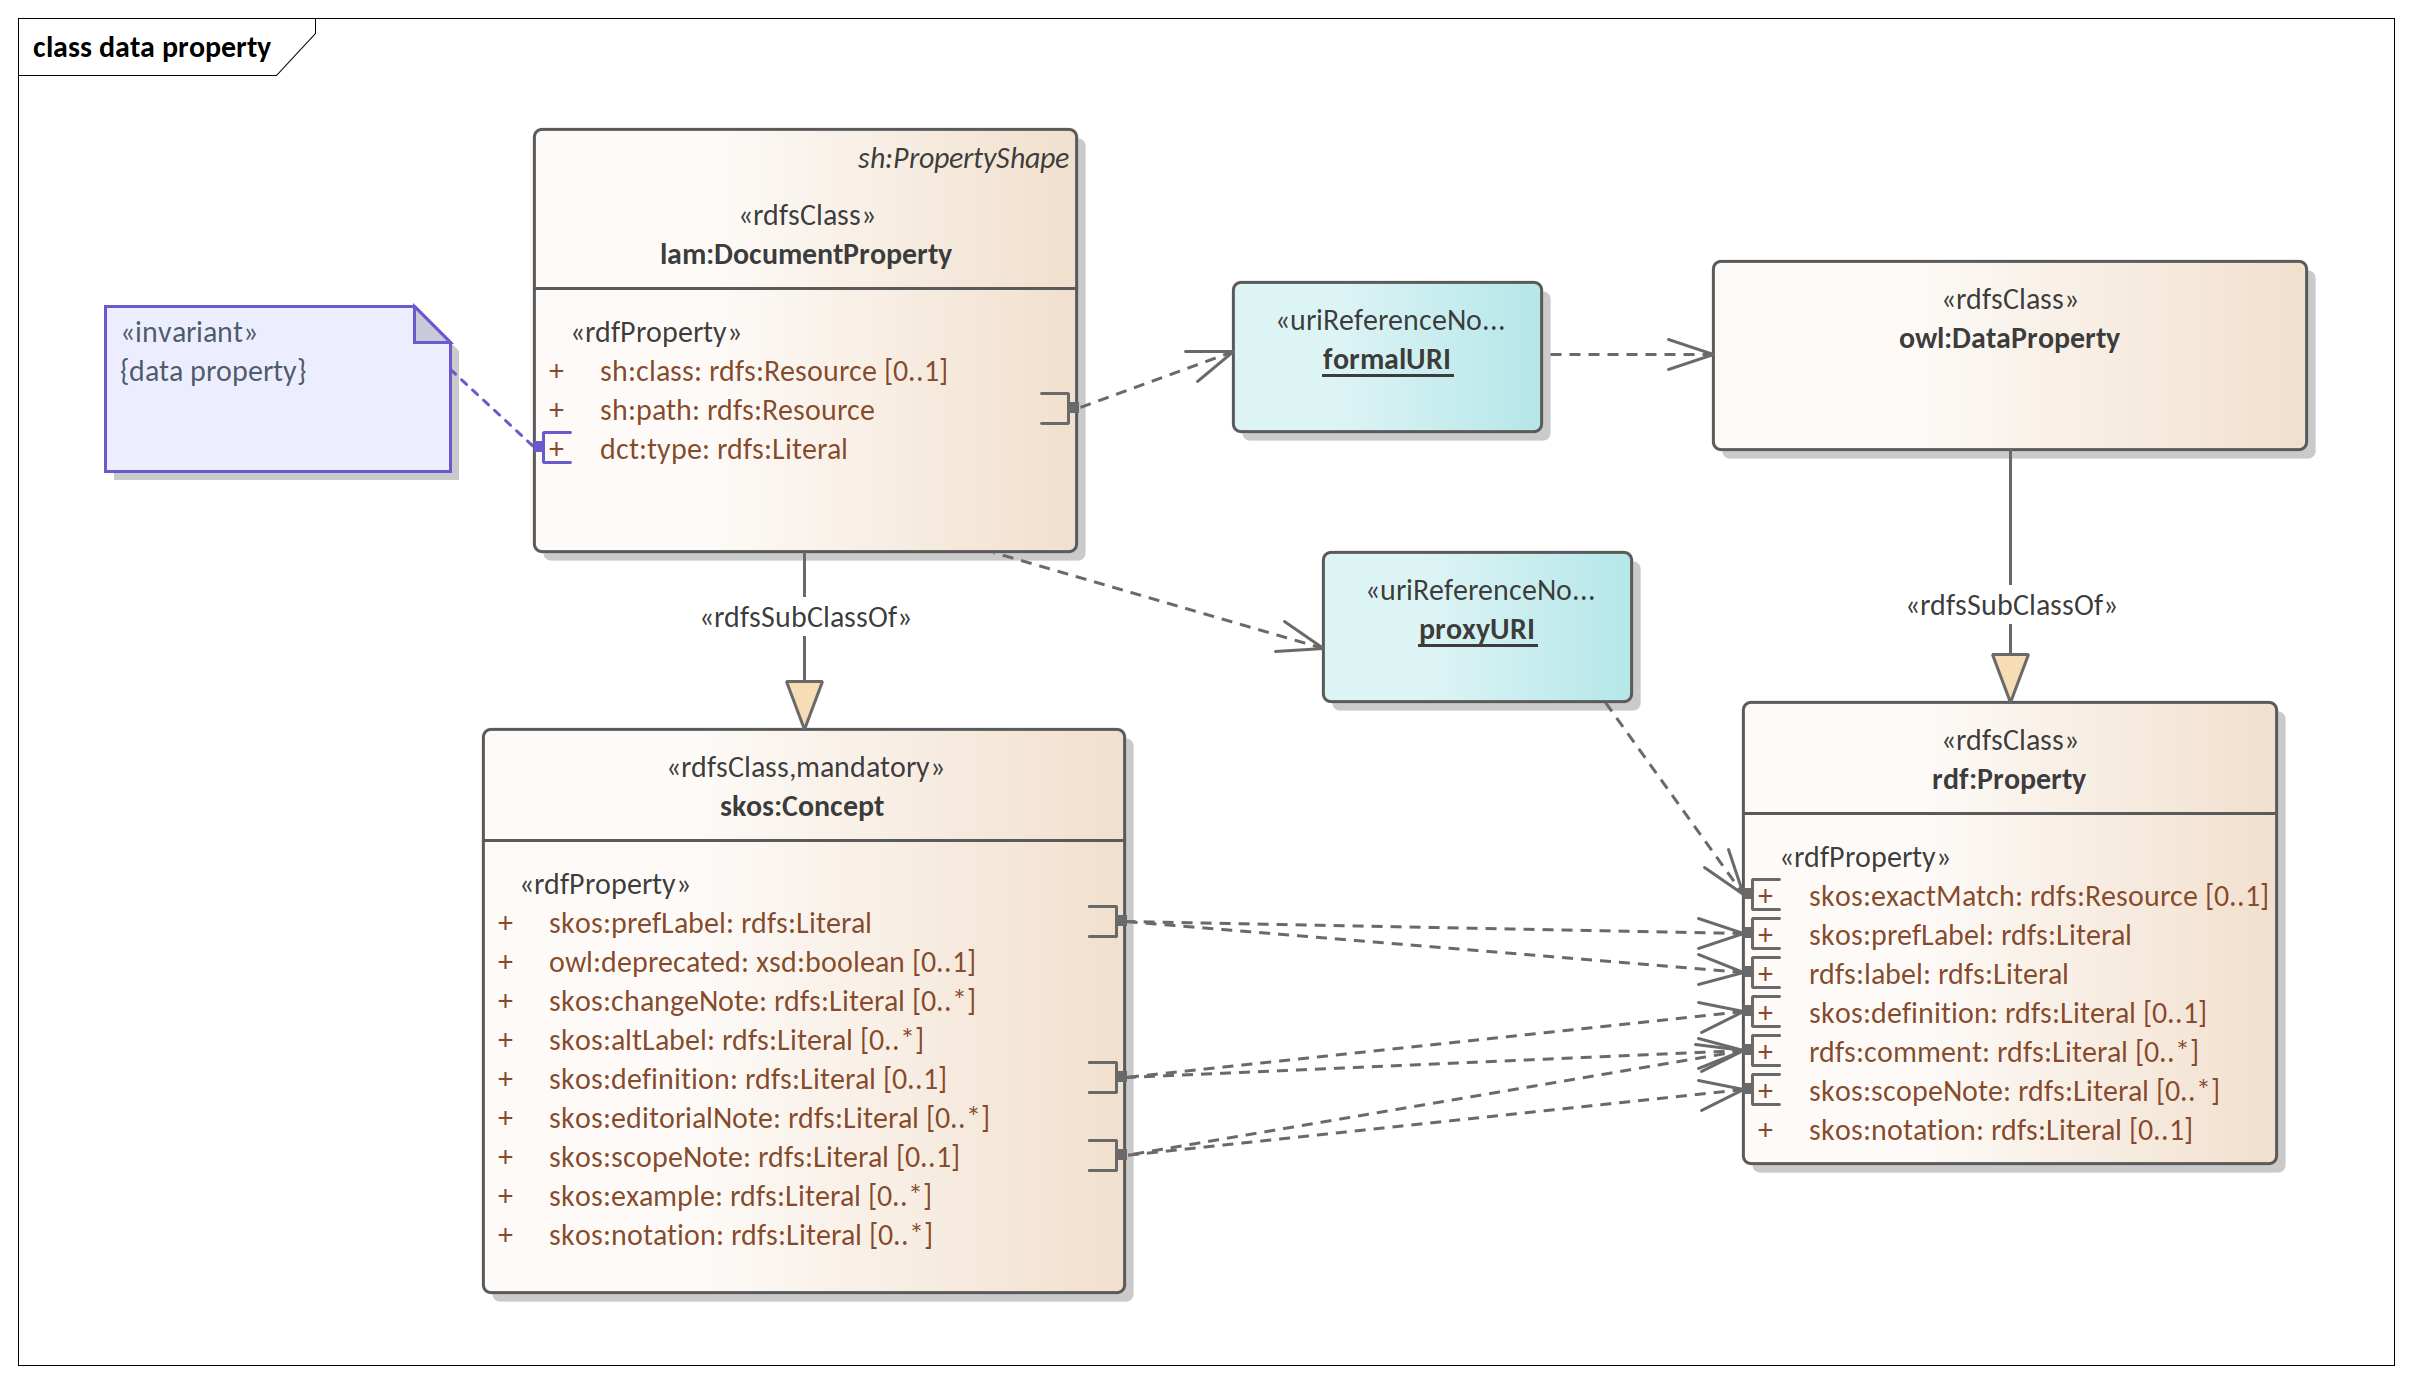
\includegraphics[width=15cm]{images/data-property.png}
		\caption{Representation of mapping lam:DocumentProperty to owl:DataProperty and owl:ObjectProperty}
		\label{fig:mapping-property-data}
	\end{figure}

	lam:DocumentProperty class is used to represent attributes and relations of the LAM entities commonly called properties. When a formal representation in OWL language is generated, unlike RDFS, we need to distinguish between properties that take a data type and those that take an URI as their values, i.e. the property range. To aid this decision lam:DocumentProperty already has the attribute \textit{dct:type}, which, as define in the Excel structure conventions\footnote {Costetchi E., 2019, The structure of Excel workbook for bootstrapping the Legal Analysis Methodology descriptions}, has two possible values: \textit{data property} and \textit{object property}. 
	In Figure \ref{fig:mapping-property-data} this is represented as an invariant constraint on the dct:type property. 
	
	lam:DocumentProperty constitutes a proxy definition to already existent formal properties mostly defined in the Common Data Model (CDM) ontology, SKOS or other models. For this reason, we call the former a \textit{proxy} while the latter a \textit{formal} property. The link between the two is established \textit{lam:path} attribute. 

	When the OWL property is created the URI used is the one given by the \textit{lam:path} attribute, in a way redefining, or rather extending the formal definition of an existent model. The inverse link is maintained by using \textit{skos:exactMatch} attribute in the owl:DataProperty pointing to the URI of the lam:DocumentProperty. In Figure \ref{fig:mapping-property-data} these correspondences are traced using \textit{uriReferenceNode} called \textit{formalURI} and \textit{proxyURI}. This transformation can be written as a SPARQL query that is provided in Listing \ref{lst:sparql-formal-proxy}. 
	
\begin{lstlisting}[language=SPARQL, captionpos=b, caption={The transformation SPARQL query for property formal definition}, label=lst:sparql-formal-proxy]
PREFIX skos: <http://www.w3.org/2004/02/skos/core#>
PREFIX dct: <http://purl.org/dc/terms/>
PREFIX rdf: <http://www.w3.org/1999/02/22-rdf-syntax-ns#>
PREFIX owl: <http://www.w3.org/2002/07/owl#>
PREFIX sh: <http://www.w3.org/ns/shacl#>

CONSTRUCT { 
	?uri a ?type .
	?uri skos:exactMatch ?p .
	#?p skos:exactMatch ?uri .
} 
WHERE { 
	?p a skos:Concept .
	?p sh:path ?uri .
	OPTIONAL {?p dct:type ?literalType . }  
	
	BIND ( 
	IF(!bound(?literalType), rdf:Property,    
	IF ( contains(?literalType,"data"), owl:DatatypeProperty,
	IF( contains(?literalType,"object"), owl:ObjectProperty, rdf:Property ))) as ?type)
}
\end{lstlisting}

	A set of editorial attributes inherited from the skos:Concept (skos:prefLabel, skos:definition, skos:scopeNote and skos:editorialNote) are transferred, as such, into a similar set of editorial attributes inherited from the rdfs:Property. This transformation can be written as a SPARQL query that is provided in Listing \ref{lst:sparql-property-editorial}.
	
\begin{lstlisting}[language=SPARQL, captionpos=b, caption={The transformation SPARQL query for editorial part of the LAM document properties}, label=lst:sparql-property-editorial]	
PREFIX skos: <http://www.w3.org/2004/02/skos/core#>
PREFIX dct: <http://purl.org/dc/terms/>
PREFIX rdf: <http://www.w3.org/1999/02/22-rdf-syntax-ns#>
PREFIX owl: <http://www.w3.org/2002/07/owl#>
PREFIX sh: <http://www.w3.org/ns/shacl#>
PREFIX rdfs: <http://www.w3.org/2000/01/rdf-schema#>
prefix xsd: <http://www.w3.org/2001/XMLSchema#>

CONSTRUCT { 
	?uri skos:prefLabel  ?prefLabel .    
	
	?uri rdfs:label  ?prefLabel .  
	
	?uri skos:definition  ?definition .  
	?uri skos:editorialNote  ?editorialNote .
	?uri skos:scopeNote  ?scopeNote .
	?uri skos:historyNote  ?historyNote .
	?uri skos:notation ?notation .
	
	?uri rdfs:comment  ?definition .  
	?uri rdfs:comment  ?editorialNote .
	?uri rdfs:comment  ?scopeNote .
	?uri rdfs:comment  ?historyNote .
	?uri rdfs:comment ?notation .
	
	# when the propoerty definition is undated 
	?uri dct:modified ?created .
	# fixed creation date
	#?uri dct:created "2019-08-27"^^xsd:date .
} 
WHERE { 
	?p a skos:Concept .
	?p sh:path ?uri .
	
	OPTIONAL {
		?p skos:prefLabel  ?prefLabel .
	}    
	OPTIONAL {
		?p skos:definition  ?definition .
	}
	OPTIONAL {
		?p skos:editorialNote  ?editorialNote .
	}
	OPTIONAL {
		?p skos:scopeNote  ?scopeNote .
	}
	OPTIONAL {
		?p skos:historyNote  ?historyNote .
	}
	OPTIONAL {
		?p skos:notation ?notation .
	}
	OPTIONAL {
		?p dct:created ?created .
	}
}
\end{lstlisting}

%\begin{figure}[h]
%	\centering
%	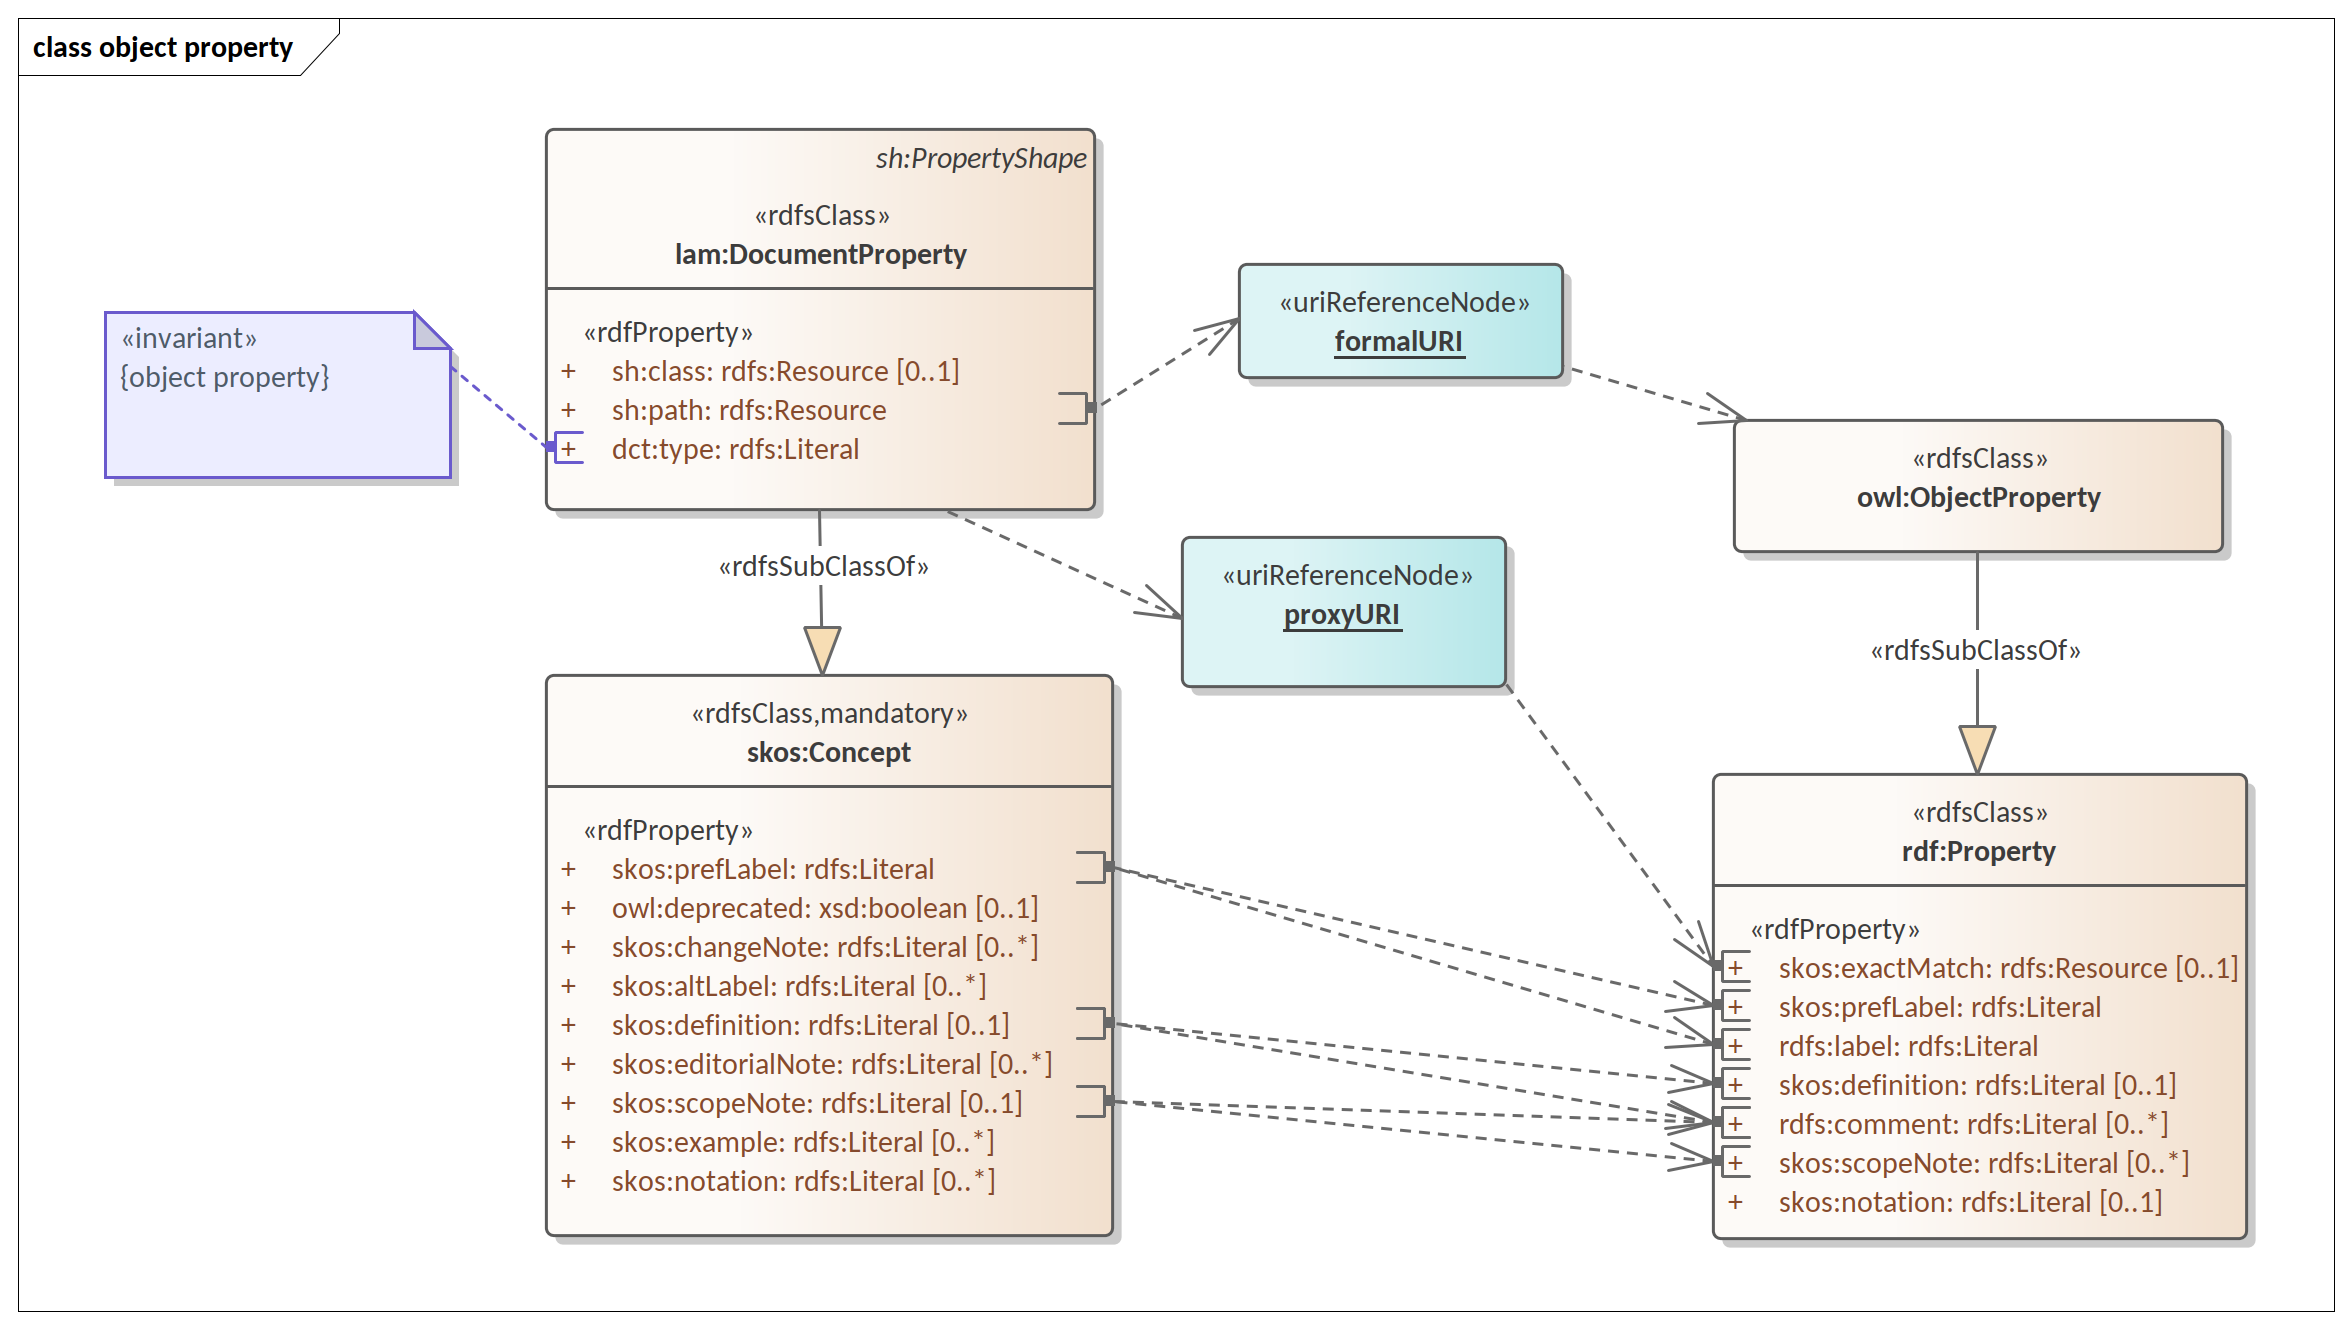
\includegraphics[width=15cm]{images/object-property.png}
%	\caption{Representation of mapping lam:DocumentProperty to owl:DataProperty and owl:ObjectProperty}
%	\label{fig:mapping-property-object}
%\end{figure}

\subsection{LAM class definition}

	This section explains how to generate OWL definitions for the legal document classes by transforming instances of  lam:LegalDocumentClass. Figure \ref{fig:mapping-class} provides a visual representation of the mapping rules.

	\begin{figure}[h]
		\centering
		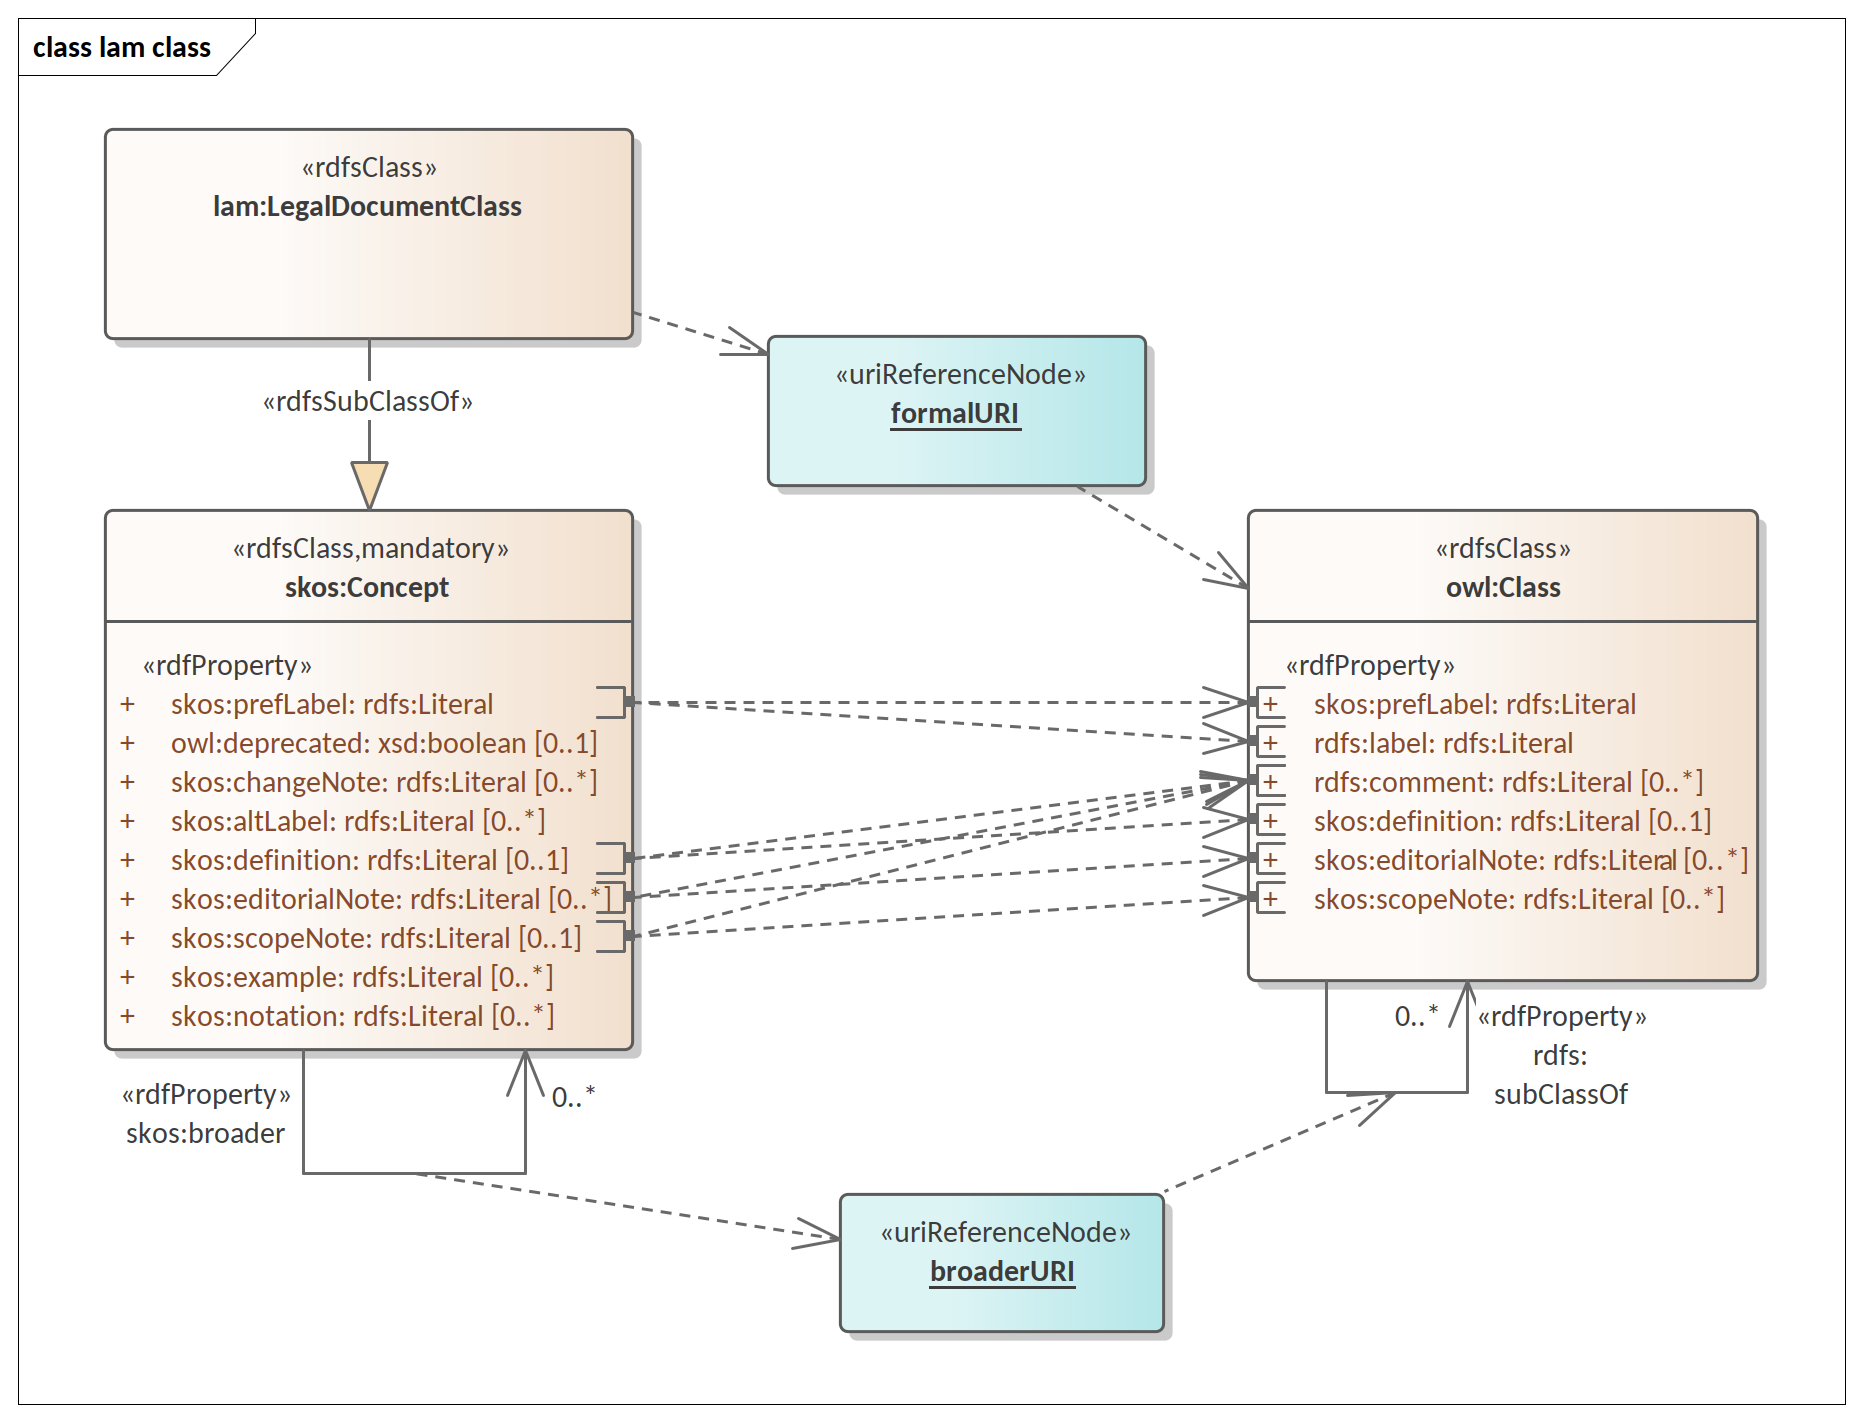
\includegraphics[width=15cm]{images/lam-class.png}
		\caption{Representation of mapping lam:LegalDocumentClass to owl:Class}
		\label{fig:mapping-class}
	\end{figure}

	There is a straight forward isomorphism between the lam:LegalDocumentClass class and its formal definition as a owl:Class. The URIs of the legal document classes are maintained in the transformation. 
	
	The editorial attributes inherited from the skos:Concept (skos:prefLabel, skos:definition, skos:scopeNote and skos:editorialNote) are transferred, as such, into a similar set of editorial attributes in the owl:Class. 
	
	The \textit{skos:broader} property, used for building conceptual hierarchies is turned into \textit{rdfs:subClassOf} property, which defines formal class hierarchies.
	
	This transformation can be written as a SPARQL query that is provided in Listing \ref{lst:sparql-legal-document}. 

	\begin{lstlisting}[language=SPARQL, captionpos=b, caption={The transformation SPARQL query for LAM legal document classes}, label=lst:sparql-legal-document]
PREFIX skos: <http://www.w3.org/2004/02/skos/core#>
PREFIX dct: <http://purl.org/dc/terms/>
PREFIX rdf: <http://www.w3.org/1999/02/22-rdf-syntax-ns#>
PREFIX owl: <http://www.w3.org/2002/07/owl#>
PREFIX sh: <http://www.w3.org/ns/shacl#>
PREFIX rdfs: <http://www.w3.org/2000/01/rdf-schema#>
prefix lamd: <http://publications.europa.eu/resources/authority/lam/>

CONSTRUCT { 
	?c a owl:Class ;
		rdfs:subClassOf lamd:LAMLegalDocument ;
		dct:modified ?created ;
		
		skos:prefLabel ?label ;
		rdfs:label ?label ;
		
		rdfs:comment ?example ;
		rdfs:comment ?editorialNote ;
		rdfs:comment ?definition ;
		
		skos:definition ?definition ;
		skos:editorialNote ?editorialNote ;
		skos:scopeNote ?scopeNote ;
		
		rdfs:subClassOf ?superClass ;
	.
} 
WHERE { 
	?c a skos:Concept .  
	OPTIONAL {
		?c dct:created ?created ;
	}	
	OPTIONAL {
		?c skos:editorialNote ?editorialNote ;
	}
	OPTIONAL {
		?c skos:example ?example ;
	}
	OPTIONAL {
		?c skos:definition ?definition ;
	}  
	OPTIONAL {
		?c skos:scopeNote ?scopeNote ;
	}    
	OPTIONAL {
		?c skos:prefLabel ?label ;
	}
	OPTIONAL {
		?c skos:broader ?superClass ;
	}
}
\end{lstlisting}

\subsection{LAM class restriction definition}

	This section explains how to generate OWL class restrictions for the legal document classes by transforming instances of  lam:PropertyConfiguration lam:LegalDocumentClass. Figure \ref{fig:mapping-class} provides a visual representation of the mapping rules.
	
	\begin{figure}[h]
		\centering
		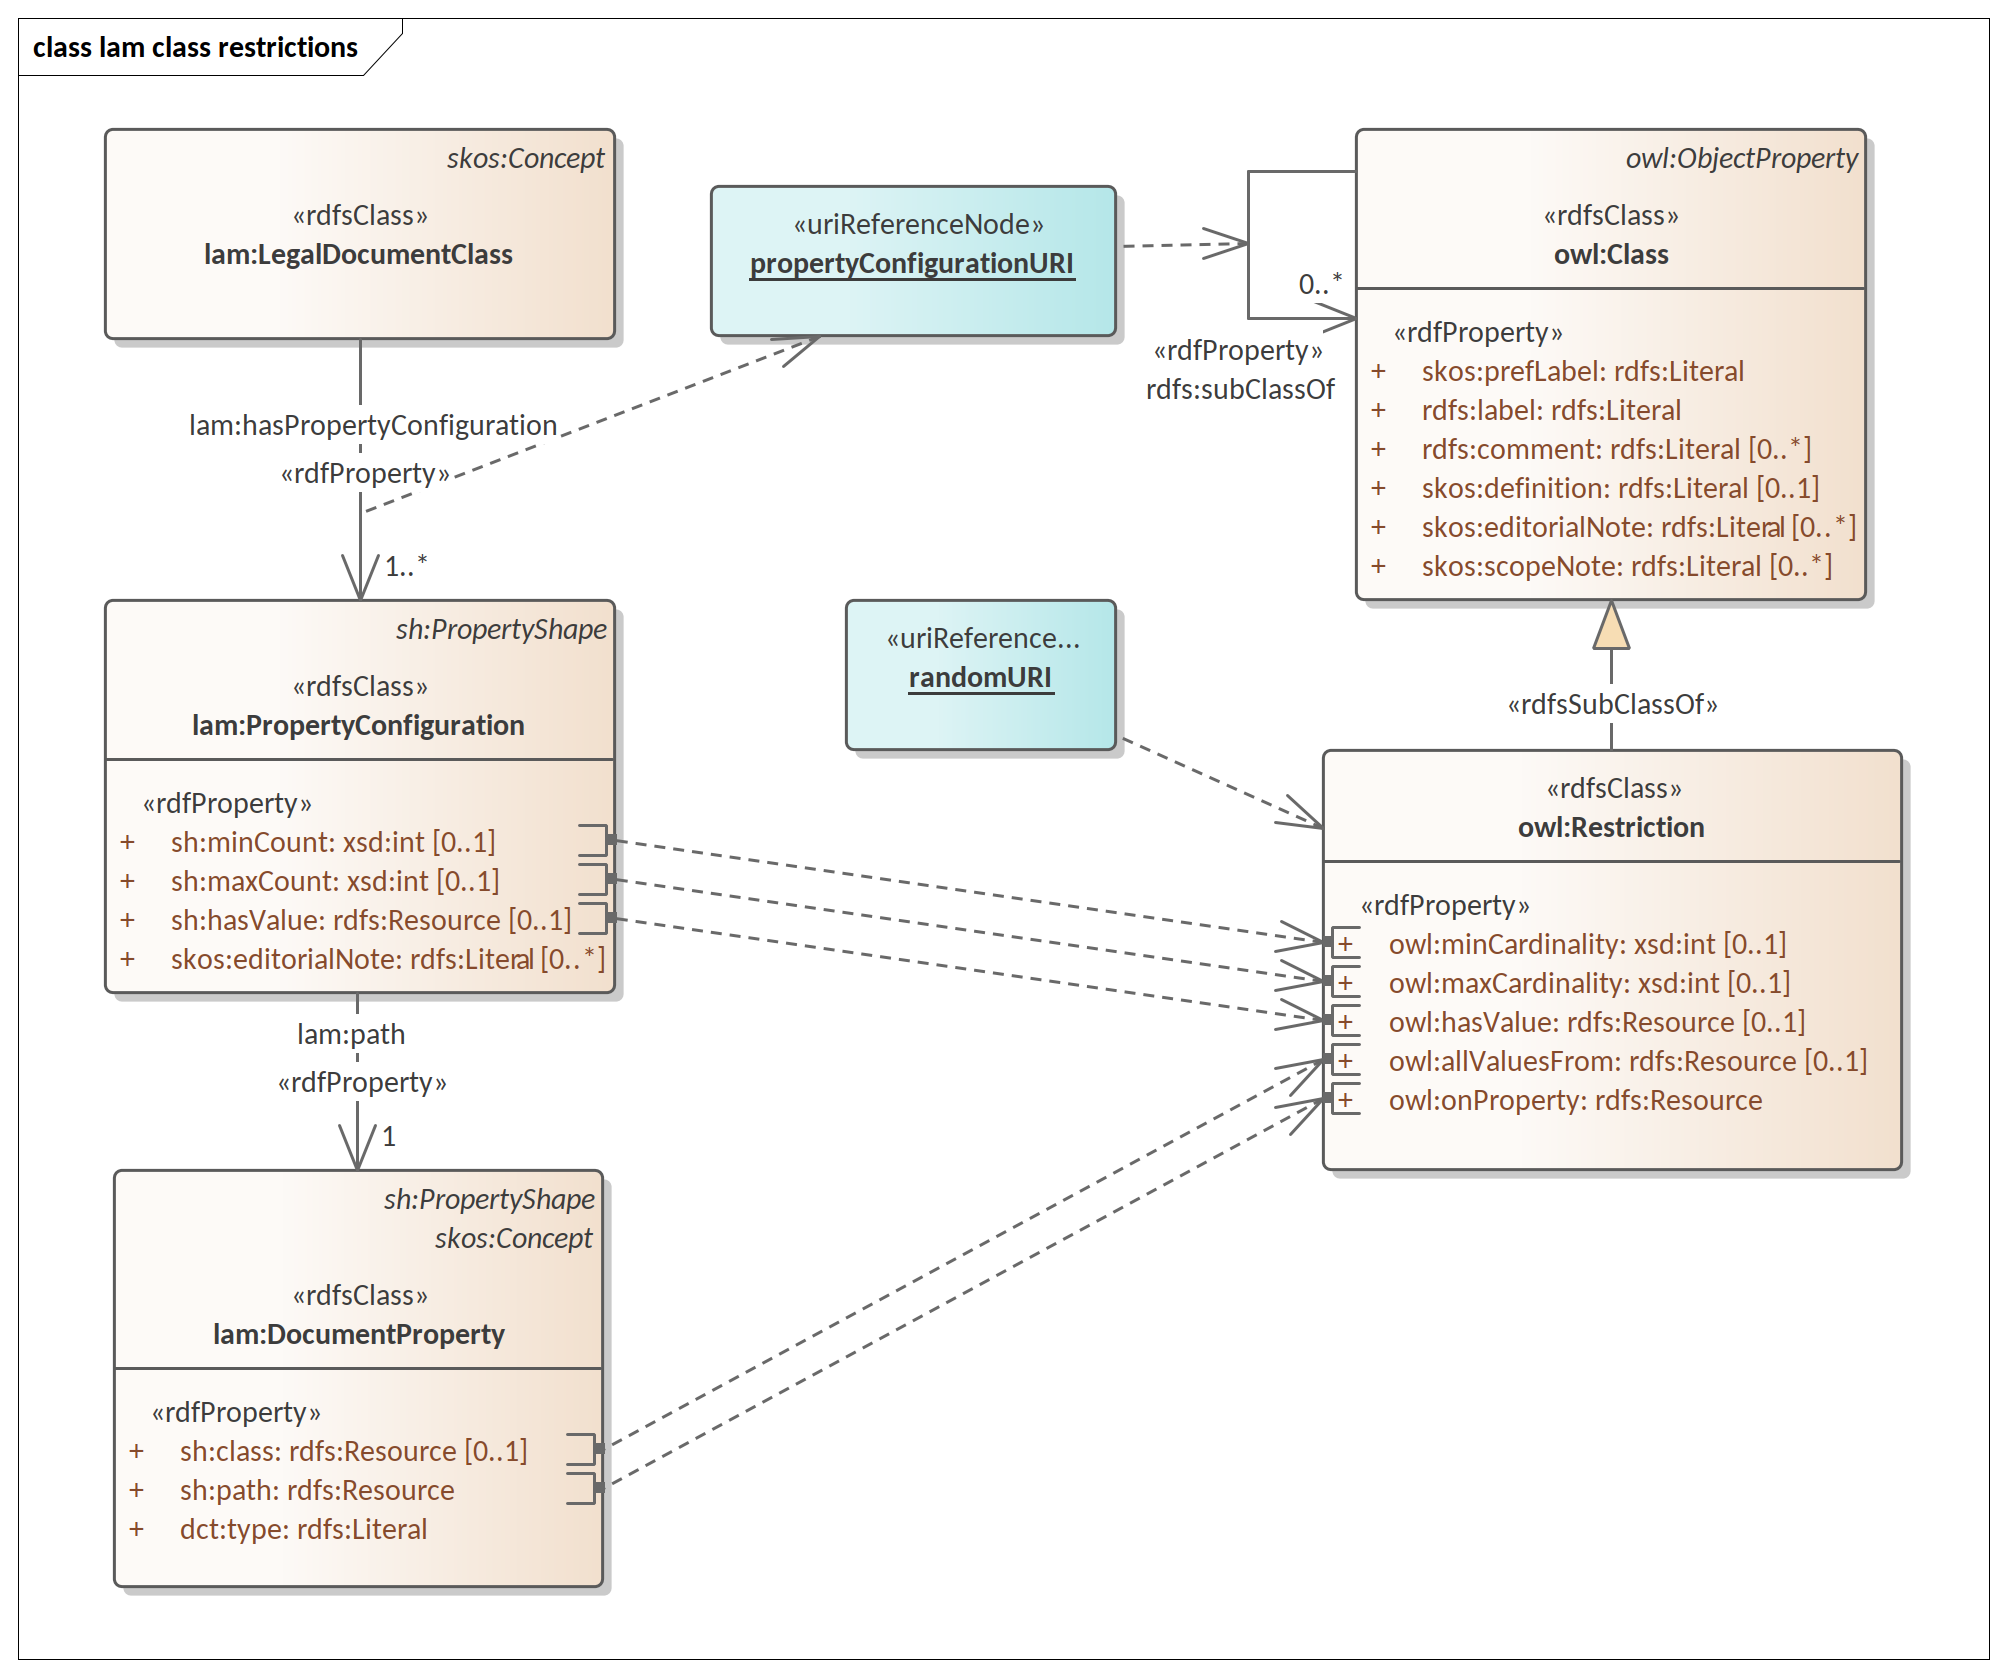
\includegraphics[width=15cm]{images/lam-class-restrictions.png}
		\caption{Representation of mapping lam:LegalDocumentClass property configurations to owl:Class restrictions}
		\label{fig:mapping-restriction}
	\end{figure}	

	The property configurations are turned into restriction classes. Formally, the restrictions act as anonymous super-classes for the document classes. This is represented in Figure \ref{fig:mapping-restriction} by linking \textit{lam:hasPropertyConfiguration} to \textit{rdfs:subClassOf} properties. 
	
	The configuration, for a \textit{lam:path} proxy property, provides three types of restrictions: specific value (\textit{sh:value}), minimum (\textit{sh:minCount}) and maximum cardinality (\textit{sh:maxCount}). They translate into the corresponding OWL properties: \textit{owl:hasValue}, \textit{owl:minCardinality} and \textit{owl:maxCardinality}.
	
	As mentioned above, the restriction specification is defined on a proxy property. But in the formal specification we need to specify the formal property. That is why we follow the link and take it from the \textit{sh:path} attribute in the lam:DocumentProperty and map it to \textit{owl:onProperty} attribute in the owl:Restriction class. Here is also available an additional constraint, that of range class (\textit{sh:class}), which translates into \textit{owl:allValuesFrom} attribute. 
	
	This transformation can be written as a SPARQL query that is provided in Listing \ref{lst:sparql-class-restriction}.  
	
	\begin{lstlisting}[language=SPARQL, captionpos=b, caption={The transformation SPARQL query for LAM legal document class restrictions}, label=lst:sparql-class-restriction]
PREFIX skos: <http://www.w3.org/2004/02/skos/core#>
PREFIX dct: <http://purl.org/dc/terms/>
PREFIX rdf: <http://www.w3.org/1999/02/22-rdf-syntax-ns#>
PREFIX owl: <http://www.w3.org/2002/07/owl#>
PREFIX sh: <http://www.w3.org/ns/shacl#>
PREFIX rdfs: <http://www.w3.org/2000/01/rdf-schema#>
prefix lam: <http://publications.europa.eu/ontology/lam-skos-ap#>
prefix lamd: <http://publications.europa.eu/resources/authority/lam/>

# construct the class restrictions
CONSTRUCT { 
	?c a owl:Class ;
	rdfs:subClassOf ?minCountIRI ;
	rdfs:subClassOf ?valueIRI ;
	rdfs:subClassOf ?maxCountIRI ;
	rdfs:subClassOf ?rangeRestrictionIRI ;
	.
	
	?minCountIRI a owl:Restriction ;
	owl:onProperty ?constrainedProperty ;    
	rdfs:label ?minCountStr;
	owl:minCardinality ?minCount .
	
	?valueIRI a owl:Restriction ;
	owl:onProperty ?constrainedProperty ;
	rdfs:label ?valueStr ;
	owl:hasValue ?value .
	
	?maxCountIRI a owl:Restriction ;
	owl:onProperty ?constrainedProperty ;
	rdfs:label ?maxCountStr ;
	owl:maxCardinality ?maxCount .
	
	?rangeRestrictionIRI a owl:Restriction ;
	owl:onProperty ?constrainedProperty ;	
	rdfs:label ?rangeRestrictionStr ;
	owl:allValuesFrom ?rangeRestriction .
	
} 
WHERE { 
	# select document class
	?c a skos:Concept . 
	
	# select the Property Configurations of each class
	?c lam:hasPropertyConfiguration ?propertyConfiguration .  
	?propertyConfiguration lam:path ?constrainedPropertyProxy .
	
	# get the constraints
	OPTIONAL {
		?propertyConfiguration sh:minCount ?minCount .
	}
	OPTIONAL {
		?propertyConfiguration sh:maxCount ?maxCount .
	}
	OPTIONAL {
		?propertyConfiguration sh:value ?value .
	}	
	
	# from the property configuration get the proxy propeorty and termine the real property
	?constrainedPropertyProxy sh:path ?constrainedProperty .  
	
	# eventually take the property range restriction
	OPTIONAL {
		?constrainedPropertyProxy sh:class ?rangeRestriction .
	}
	
	# generating some IRIs
	BIND ( IRI( concat(str(lamd:), MD5(concat(str(?constrainedProperty),str(?minCount))))) 
	as ?minCountIRI)
	
	BIND ( IRI( concat(str(lamd:), MD5(concat(str(?constrainedProperty),str(?maxCount) ) ))) 
	as ?maxCountIRI)
	
	BIND ( IRI( concat(str(lamd:), MD5(concat(str(?constrainedProperty),str(?value) ) ))) 
	as ?valueIRI)
	
	BIND ( IRI( concat(str(lamd:), MD5(concat(str(?constrainedProperty),str(?rangeRestriction) ) ))) 
	as ?rangeRestrictionIRI)	
	
	BIND (  concat(str("Restriction on "), concat(replace( str(?constrainedProperty), 
		"http://publications.europa.eu/ontology/cdm#", "cdm:" )," to min ",str(?minCount))) 
	as ?minCountStr)
	
	BIND (  concat(str("Restriction on "), concat(replace( str(?constrainedProperty), 
		"http://publications.europa.eu/ontology/cdm#", "cdm:" )," to max ",str(?maxCount) ) ) 
	as ?maxCountStr)
	
	BIND (  concat(str("Restriction on "), concat(replace( str(?constrainedProperty), 
		"http://publications.europa.eu/ontology/cdm#", "cdm:" )," to value ",str(?value) ) ) 
	as ?valueStr)
	
	BIND (  concat(str("Restriction on "), concat(replace( str(?constrainedProperty), 
		"http://publications.europa.eu/ontology/cdm#", "cdm:" )," to class ", str(?rangeRestriction) ) ) 
	as ?rangeRestrictionStr)
}
	\end{lstlisting}
	
	Note that the above query segregates each type of restriction into a separate restriction instance. This is valuable separation fo concerns and allows for a limited number of restrictions to be reused. Having this done like that will help in the future classification exercises to distinguish clusters of legal document classes. 
	
\subsection{LAM class shape definition}
	
	This section explains how to generate SHACL class restrictions for the legal document classes by transforming instances of  lam:PropertyConfiguration lam:LegalDocumentClass. 
	
	This transformation is isomorphic with the class restriction structure described in the section above. The owl:Restriction class is replaced by the \textit{sh:PropertyShape} while the the relation to the document class in no longer one of sub-classification but is \textit{sh:property}.
	
	In the SHACL constraint specification, the legal document class, besides being an OWL class, receives an additional type, that of \textit{sh:NodeShape}. 
	
	This transformation can be written as a SPARQL query that is provided in Listing \ref{lst:sparql-class-constraint}. 

	\begin{lstlisting}[language=SPARQL, captionpos=b, caption={The transformation SPARQL query for LAM legal document class restrictions}, label=lst:sparql-class-constraint]	
PREFIX skos: <http://www.w3.org/2004/02/skos/core#>
PREFIX dct: <http://purl.org/dc/terms/>
PREFIX rdf: <http://www.w3.org/1999/02/22-rdf-syntax-ns#>
PREFIX owl: <http://www.w3.org/2002/07/owl#>
PREFIX sh: <http://www.w3.org/ns/shacl#>
PREFIX rdfs: <http://www.w3.org/2000/01/rdf-schema#>
prefix lam: <http://publications.europa.eu/ontology/lam-skos-ap#>
prefix lamd: <http://publications.europa.eu/resources/authority/lam/>

# construct the class restrictions
CONSTRUCT { 
	?c a sh:NodeShape ;
	sh:property ?minCountIRI ;
	sh:property ?valueIRI ;
	sh:property ?maxCountIRI ;
	sh:property ?rangeRestrictionIRI ;
	.
	
	?minCountIRI a sh:PropertyShape ;
	sh:path ?constrainedProperty ;    
	sh:name ?minCountStr;
	sh:minCount ?minCount .
	
	?valueIRI a sh:PropertyShape ;
	sh:path ?constrainedProperty ;
	sh:name ?valueStr ;
	sh:hasValue ?value .
	
	?maxCountIRI a sh:PropertyShape ;
	sh:path ?constrainedProperty ;
	sh:name ?maxCountStr ;
	sh:maxCount ?maxCount .
	
	?rangeRestrictionIRI a sh:PropertyShape ;
	sh:path ?constrainedProperty ;	
	sh:name ?rangeRestrictionStr ;
	sh:class ?rangeRestriction .
} 
WHERE { 
	# select document classes
	?c a skos:Concept . 
	#?c skos:inScheme lamd:LAMLegalDocument . # lamd:DocumentProperty  
	
	# select the Property Configurations of each class
	?c lam:hasPropertyConfiguration ?propertyConfiguration .  
	?propertyConfiguration lam:path ?constrainedPropertyProxy .
	
	# get the constraints
	OPTIONAL {
		?propertyConfiguration sh:minCount ?minCount .
	}
	OPTIONAL {
		?propertyConfiguration sh:maxCount ?maxCount .
	}
	OPTIONAL {
		?propertyConfiguration sh:value ?value .
	}
	
	
	# from the propeorty configuration get the proxy propeorty and termine the real property
	?constrainedPropertyProxy sh:path ?constrainedProperty .  
	
	# eventually take the property range restriction
	OPTIONAL {
		?constrainedPropertyProxy sh:class ?rangeRestriction .
	}
	
	# generating some IRIs
	BIND ( IRI( concat(str(lamd:), MD5(concat("-",str(?constrainedProperty),str(?minCount))))) 
	as ?minCountIRI)
	
	BIND ( IRI( concat(str(lamd:), MD5(concat("-",str(?constrainedProperty),str(?maxCount) ) ))) 
	as ?maxCountIRI)
	
	BIND ( IRI( concat(str(lamd:), MD5(concat("-",str(?constrainedProperty),str(?value) ) ))) 
	as ?valueIRI)
	
	BIND ( IRI( concat(str(lamd:), MD5(concat("-",str(?constrainedProperty),str(?rangeRestriction) ) ))) 
	as ?rangeRestrictionIRI)
	
	
	BIND (  concat(str("Constraint on "), concat(replace( str(?constrainedProperty), 
		"http://publications.europa.eu/ontology/cdm#", "cdm:" )," to min ",str(?minCount))) 
	as ?minCountStr)
	
	BIND (  concat(str("Constraint on "), concat(replace( str(?constrainedProperty), 
		"http://publications.europa.eu/ontology/cdm#", "cdm:" )," to max ",str(?maxCount) ) ) 
	as ?maxCountStr)
	
	BIND (  concat(str("Constraint on "), concat(replace( str(?constrainedProperty), 
		"http://publications.europa.eu/ontology/cdm#", "cdm:" )," to value ",str(?value) ) ) 
	as ?valueStr)
	
	BIND (  concat(str("Constraint on "), concat(replace( str(?constrainedProperty), 
		"http://publications.europa.eu/ontology/cdm#", "cdm:" )," to class ", str(?rangeRestriction) ) ) 
	as ?rangeRestrictionStr)
}
\end{lstlisting}

